
\newpage

\section{BERT}
\label{sec:bert}

Bidirectional Encoder Representations from Transformers (BERT) is a
state-of-the-art NLP embedding technique published in 2018. BERT relies on the
encoder part of the Transformer and whose objective is to generate an
unsupervised language representation model. Unlike Word2Vec, the embeddings
generated by BERT are contextualized using bidirectional representations. In the
original paper, two pre-trained BERT models trained on the English Wikipedia
(\SI{2500}{M} words) and the Toronto BookCorpus (\SI{800}{M} words) are
available:
\begin{enumerate}
\item \textbf{BERT-Base}: 12-layer Transformer, 768-hidden, 12-heads, \SI{110}{M} parameters.
\item \textbf{BERT-Large}: 24-layer Transformer, 1024-hidden, 16-heads, \SI{340}{M} parameters.
\end{enumerate}

Since these models are pre-trained based on a corpus, their use fixes the
learning vocabulary. From then on, as Word2Vec and FastText, BERT could face the
presence of OOV words. As a result of these unknown words, BERT uses an adaptive
tokenization algorithm.

\subsection{Tokenization}
\label{subsec:tokenization}

BERT uses a WordPiece tokenization algorithm for the pre-training of a
model. This tokenization proposed in 2015 by Google takes its main advantage to
not replace unknown words with a \texttt{[UNK]} special token, which implies a
loss of information about the input sequence. As an alternative to this
conversion, WordPiece uses a segmentation method which breaks down a word into
several word pieces units prefixed by \texttt{\#\#}\footnote{Except for Chinese
characters, which are surrounded by spaces before any tokenization.} and
converted into unique identifiers. From then on, this algorithm allows BERT to
learn common sub-words and does not considers OOV and rares words. As for the
vocabulary ($\simeq$ \SI{30 000}{words}), the latter is initializing itself by
taking the individual characters of a language, and adding the most frequent
combinations\footnote{For example, ``u'', followed by ``g'', would have only
been merged if the probability of ``ug'' divided by ``u'', ``g'' would have been
greater than for any other symbol pair.} of a corpus.

\begin{table}[!ht]
  \centering
  \caption{Example of Tokenization With BERT.}
  \label{tab:bert:tokenization}
  \begin{tabular}{cccccccccc}
    & The & machine & loves & embeddings. & & & & & \\
    \texttt{[CLS]} & the & machine & loves & em & \#\#bed & \#\#ding & \#\#s & . & \texttt{[SEP]} \\
    101 & 1996 & 3698 & 7459 & 7861 & 8270 & 4667 & 2015 & 1012 & 102 \\
  \end{tabular}
\end{table}

In Table \ref{tab:bert:tokenization}, the input sequence of BERT allows
receiving either one sentence (e.g., for text classification) or two sentences
(e.g., for question answering) where each of them is limited to 512
characters. Beyond this limit, it is necessary to truncate the
sentence. Finally, WordPiece uses three main special tokens:
\begin{enumerate}
\item \texttt{[CLS]}: classification token inserted at the beginning of the
  input used for prediction.
\item \texttt{[SEP]}: separator token used to indicates the end of each sentence;
\item \texttt{[PAD]}: padding token used when batching sequences of different lengths.
\end{enumerate}

\subsection{Input Embeddings}
\label{subsec:bert:input:embeddings}

Unlike Transformer, BERT accepts one or two sentences as input sentences. From
then on, BERT encodes these inputs to use them for the model pre-training.

\newpage

\begin{figure}[!ht]
  \centering
  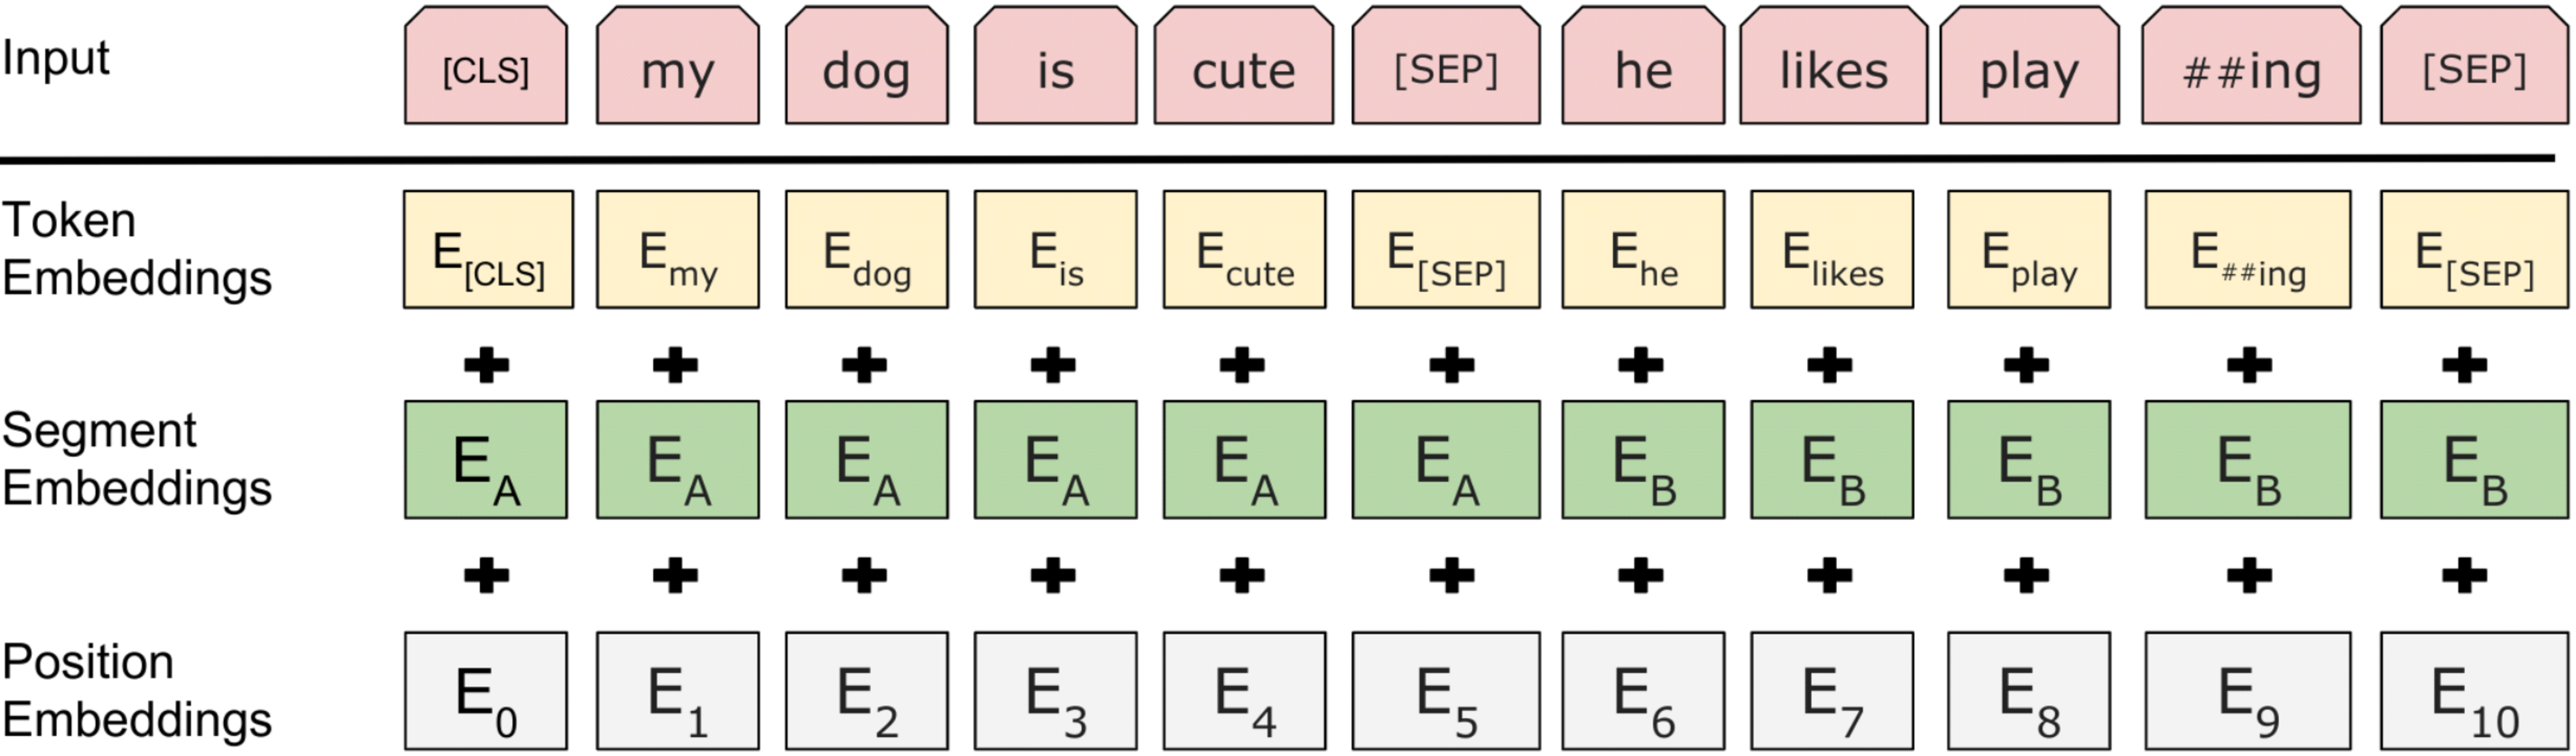
\includegraphics[width=\textwidth]{img/embedders/bert/input-embeddings}
  \caption{Example of Sentence Pair Encodding.}
  \source{\textsc{Devlin} et al. -- BERT}
  \label{fig:sentence:pair:encoding}
\end{figure}

In Figure \ref{fig:sentence:pair:encoding}, the encoding of the BERT's input
requires the sum of three vector embeddings:
\begin{enumerate}
\item \textbf{Token embeddings}: the word pieces embeddings (cf. Section
\ref{subsec:tokenization}).
\item \textbf{Segment embeddings}: the embeddings that associate a token with
its belonging sentence. In the case of a single sentence input sequence, the
vector contains only unitary values. Otherwise, the \texttt{[SEP]} token and the
tokens related to the first sentence are assigned a zero value. Those tokens of
the second sentence are assigned a unitary value.
\item \textbf{Position embeddings}: embeddings that preserve the contextual
information of the tokens by injecting their positioning into the input
embeddings, as the Transformer architecture does.
\end{enumerate}

\subsection{Pre-training}
\label{subsec:bert:pre-training}


The BERT model's pre-training gives it the ability to learn language by training
simultaneously on two unsupervised tasks: the \emph{Masked Language Model} (MLM)
and \emph{Next Sentence Prediction} (NSP). These two tasks mainly help overcome
the lack of training data and allow the model to understand better a
bidirectional representation of an input at the sentence and token level.

\subsubsection{Masked Language Model}
\label{subsubsec:bert:mlm}

MLM is the first task use by the pre-training BERT model. This task helps BERT
learn bidirectional contextual representations of tokens through the encoder
layers by predicting masked tokens from the input sequence. For this purpose,
MLM masks and predicts tokens from the input sequence. Mathematically, the
following equation defines this prediction of masked tokens.

\begin{equation}
  p\left(x_1,\dotsc,x_n\right) = \sum_{i = 1}^np\left(x_i|x_1,\dotsc,x_{i - 1}, x_{i + 1},\dotsc, x_n\right)
\label{eq:def:mlm}
\end{equation}

where each input sequence generally has \SI{15}{\percent} of its tokens hidden
according to the following subrules:
\begin{itemize}
\item a token is replaced by a \texttt{[MASK]} token in \SI{80}{\percent} of the
  cases;
\item a token is replaced randomly in \SI{10}{\percent} of the cases;
\item a token remains unchanged in \SI{10}{\percent} of the cases.
\end{itemize}

These subrules prevent the Transformer encoder from being forced to maintain a
distributive contextual representation of each input token. From then on, it is
not recommended to modify the default token masking. Too little masking would
imply a too expensive model to train, and too much masking would mean a lack of
context for a token.

\subsubsection{Next Sentence Prediction}
\label{subsubsec:bert:nsp}

The NSP is the second task use by the pre-training BERT model. This task helps
BERT learn sentence relationships by solving a binary classification problem
using Attention information shared between sentences.
\begin{table}[!ht]
  \centering
  \caption{Example of NSP With BERT.}
  \label{tab:bert:nsp}
  \begin{tabular}{lll}
    \textbf{Sentence $\mathcal{A}$} & \textbf{Sentence $\mathcal{B}$} & \textbf{Label} \\
    GNU Emacs is the best text editor. & I should use it. & \texttt{isNextSentence} \\
    GNU Emacs is the best text editor. & I have a cat. & \texttt{NotNextSentence} \\
  \end{tabular}
\end{table}

In Table \ref{tab:bert:nsp}, NSP allows the model to train itself to predict
whether sentence $\mathcal{B}$ is a continuation of sentence $\mathcal{A}$. For
this purpose, the generation of the input sequences ensures continuity of
$\mathcal{A}$ \SI{50}{\percent} of the time, labeled as \texttt{isNext}. The
rest of the time, $\mathcal{B}$ is related to a random sentence from the
provided training data set, labeled as \texttt{NotNextSentence}.

\subsubsection{Output}
\label{subsubsec:output}

Once the BERT model understands the language representation, this model is
suitable for most NLP tasks. These tasks include Neural Machine Translation,
question answering, sentiment analysis, and text summarization.
\begin{figure}[!ht]
  \centering
  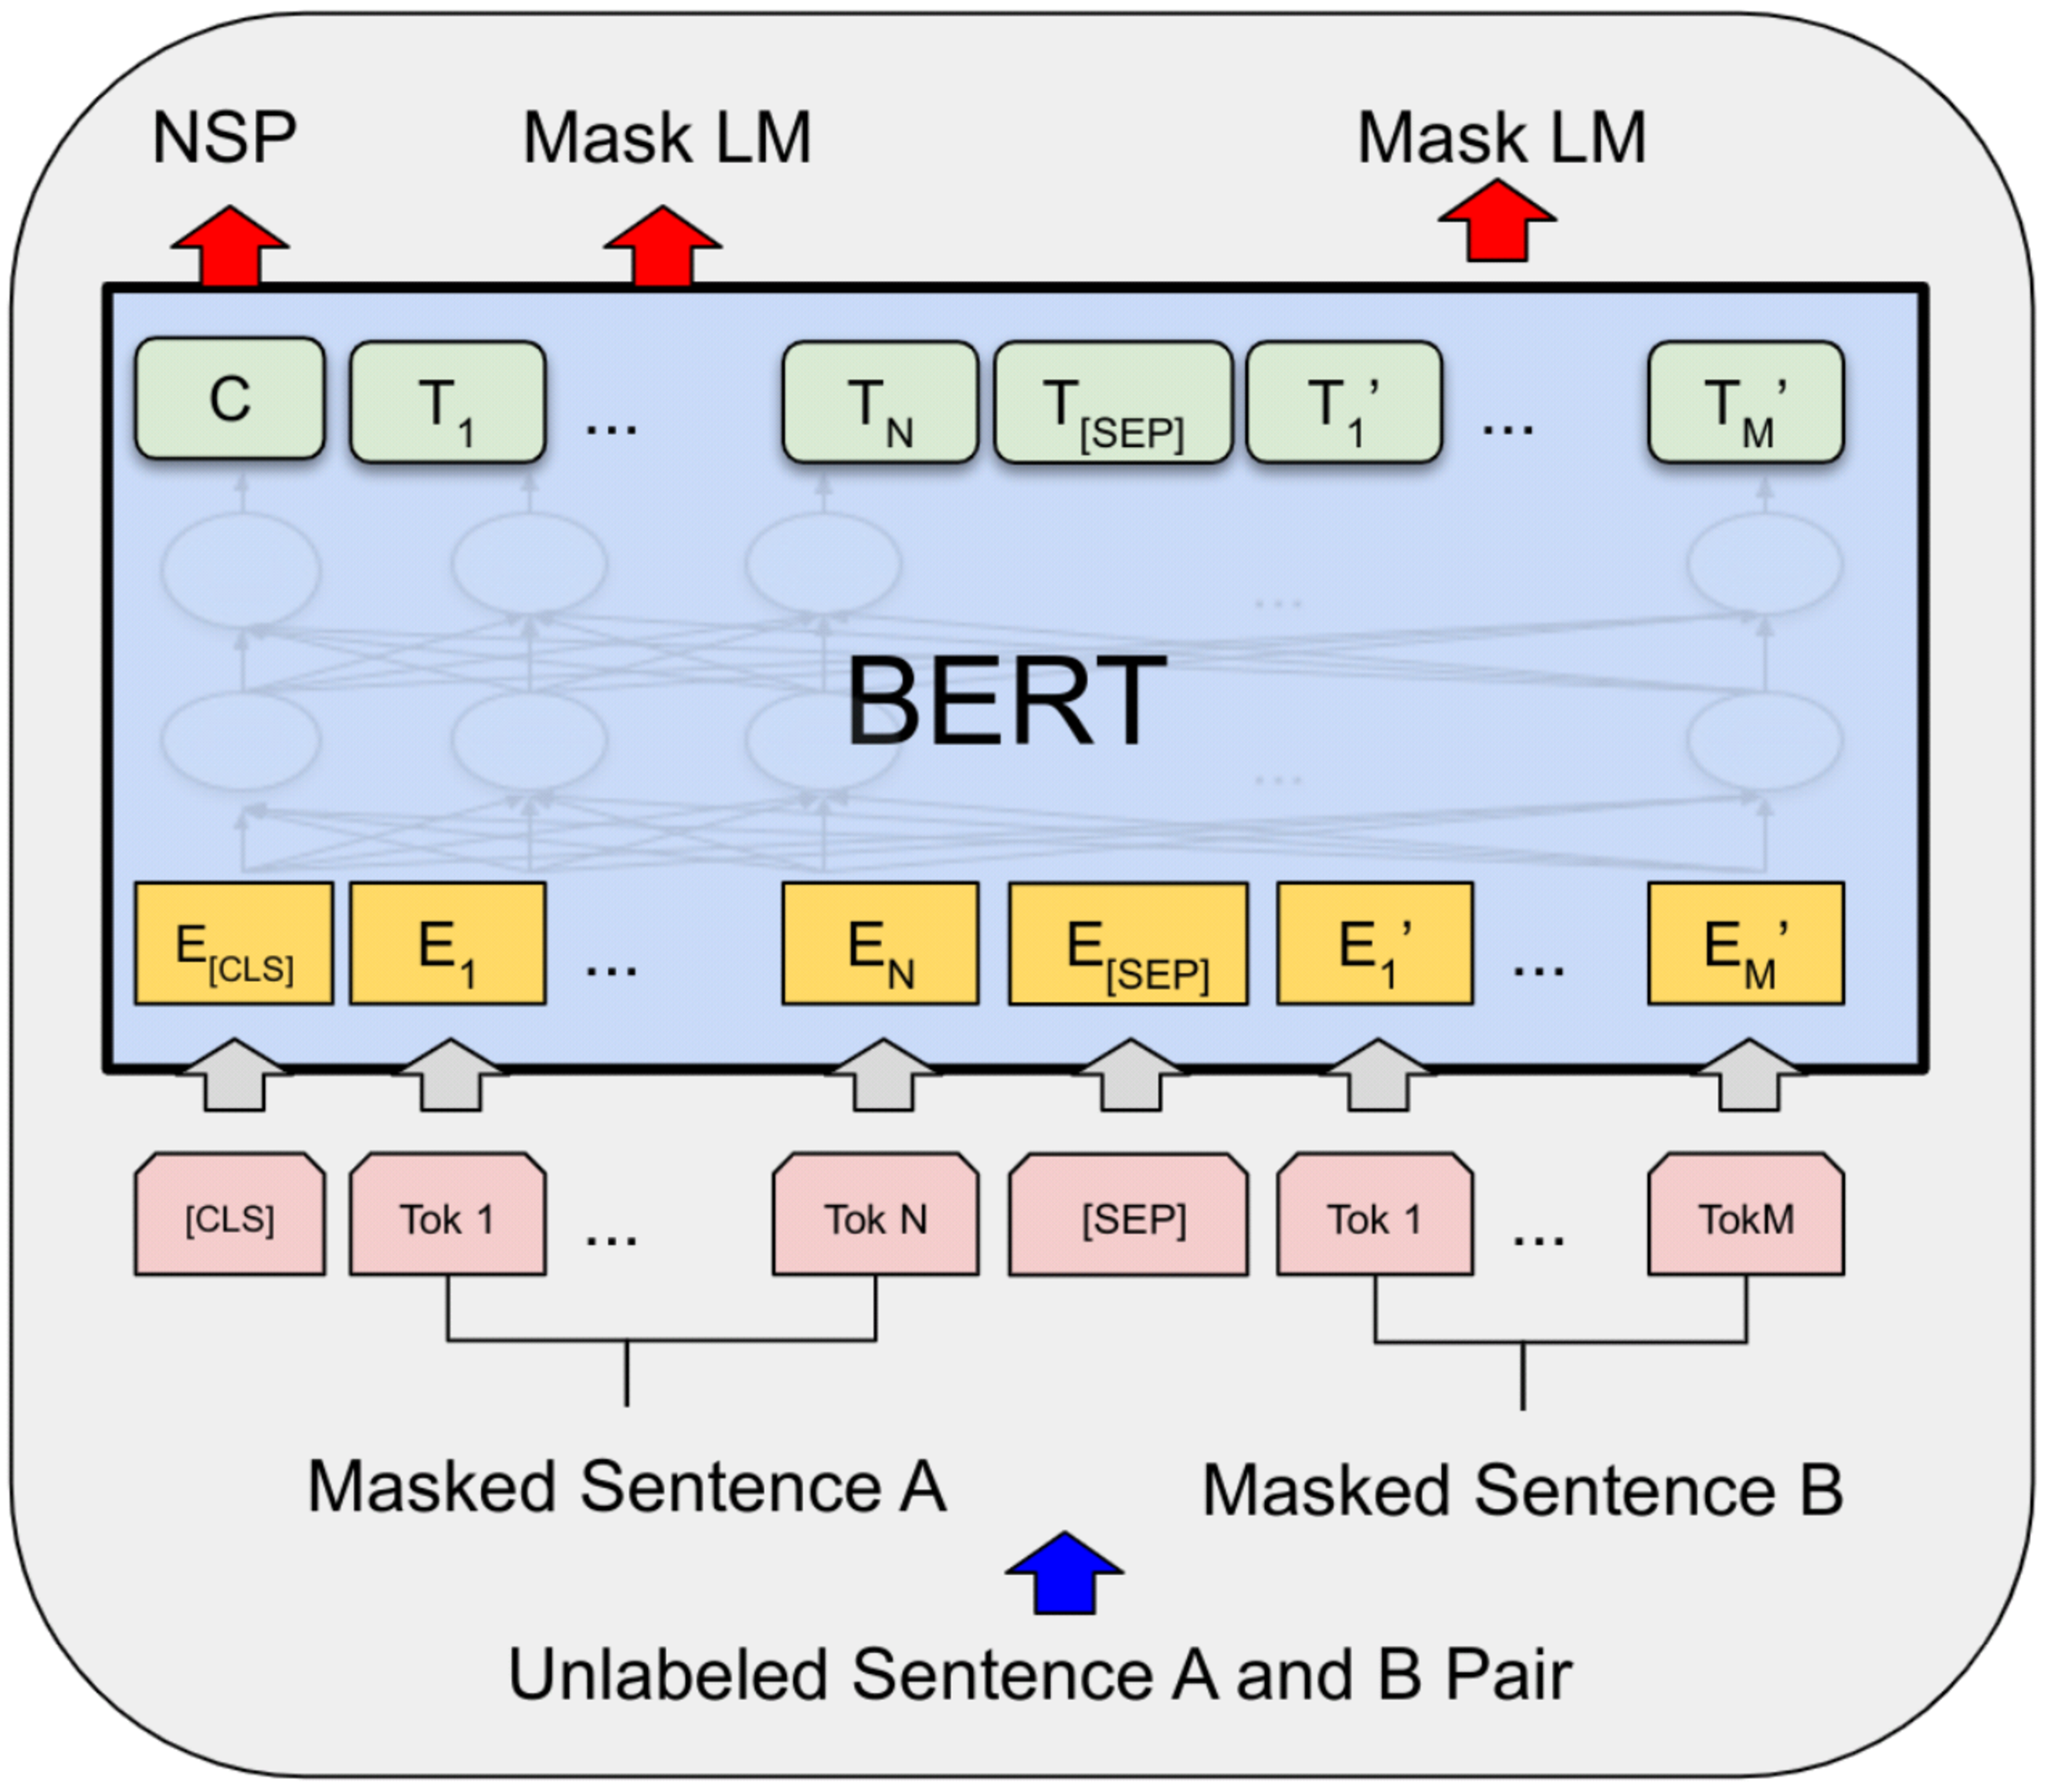
\includegraphics[width=0.6\textwidth]{img/embedders/bert/pre-training}
  \caption{Pre-Training With BERT.}
  \source{\textsc{Devlin} et al. -- BERT}
  \label{fig:pre-training}
\end{figure}

In Figure \ref{fig:pre-training}, BERT produces the hidden states of each input
token where each hidden state consists of a vector of the same size (e.g., 768
for BERT-Base) as the others, containing float numbers.  Among these hidden
states, the first position is related to the hidden state of the token
\texttt{[CLS]}. This hidden state is interesting as it determines the continuity
of two sentences, which can later be used for fine-tuning tasks.

Furthermore, the hidden states pass through a last FFN containing as many
neurons as tokens in the vocabulary used. The pre-training phase ends by
obtaining probability distribution on the hidden states using a softmax
activation function at the output of this FFN. Finally, BERT compares the
distribution of the current one-hot encoded vector token with the predicted word
and train the network using cross-entropy. It is important to note that the loss
only considers the prediction of masked tokens produced by the network to raise
awareness of the context during the network's training.

\subsection{Fine-Tuning}
\label{subsec:bert:fine-tuning}

The fine-tuning consists of training the BERT model on a specific NLP
task. Depending on the use case, either the final hidden state of the
\texttt{[CLS]} token or the hidden of the other tokens will be taken. The former
is use for classification-related tasks and the latter for more complex tasks
such as the Stanford Question Answering Dataset (SQuAD), Named Entity
Recognition (NER), and Multi-Genre Natural Language Inference (MNLI).
\begin{figure}[!ht]
  \centering
  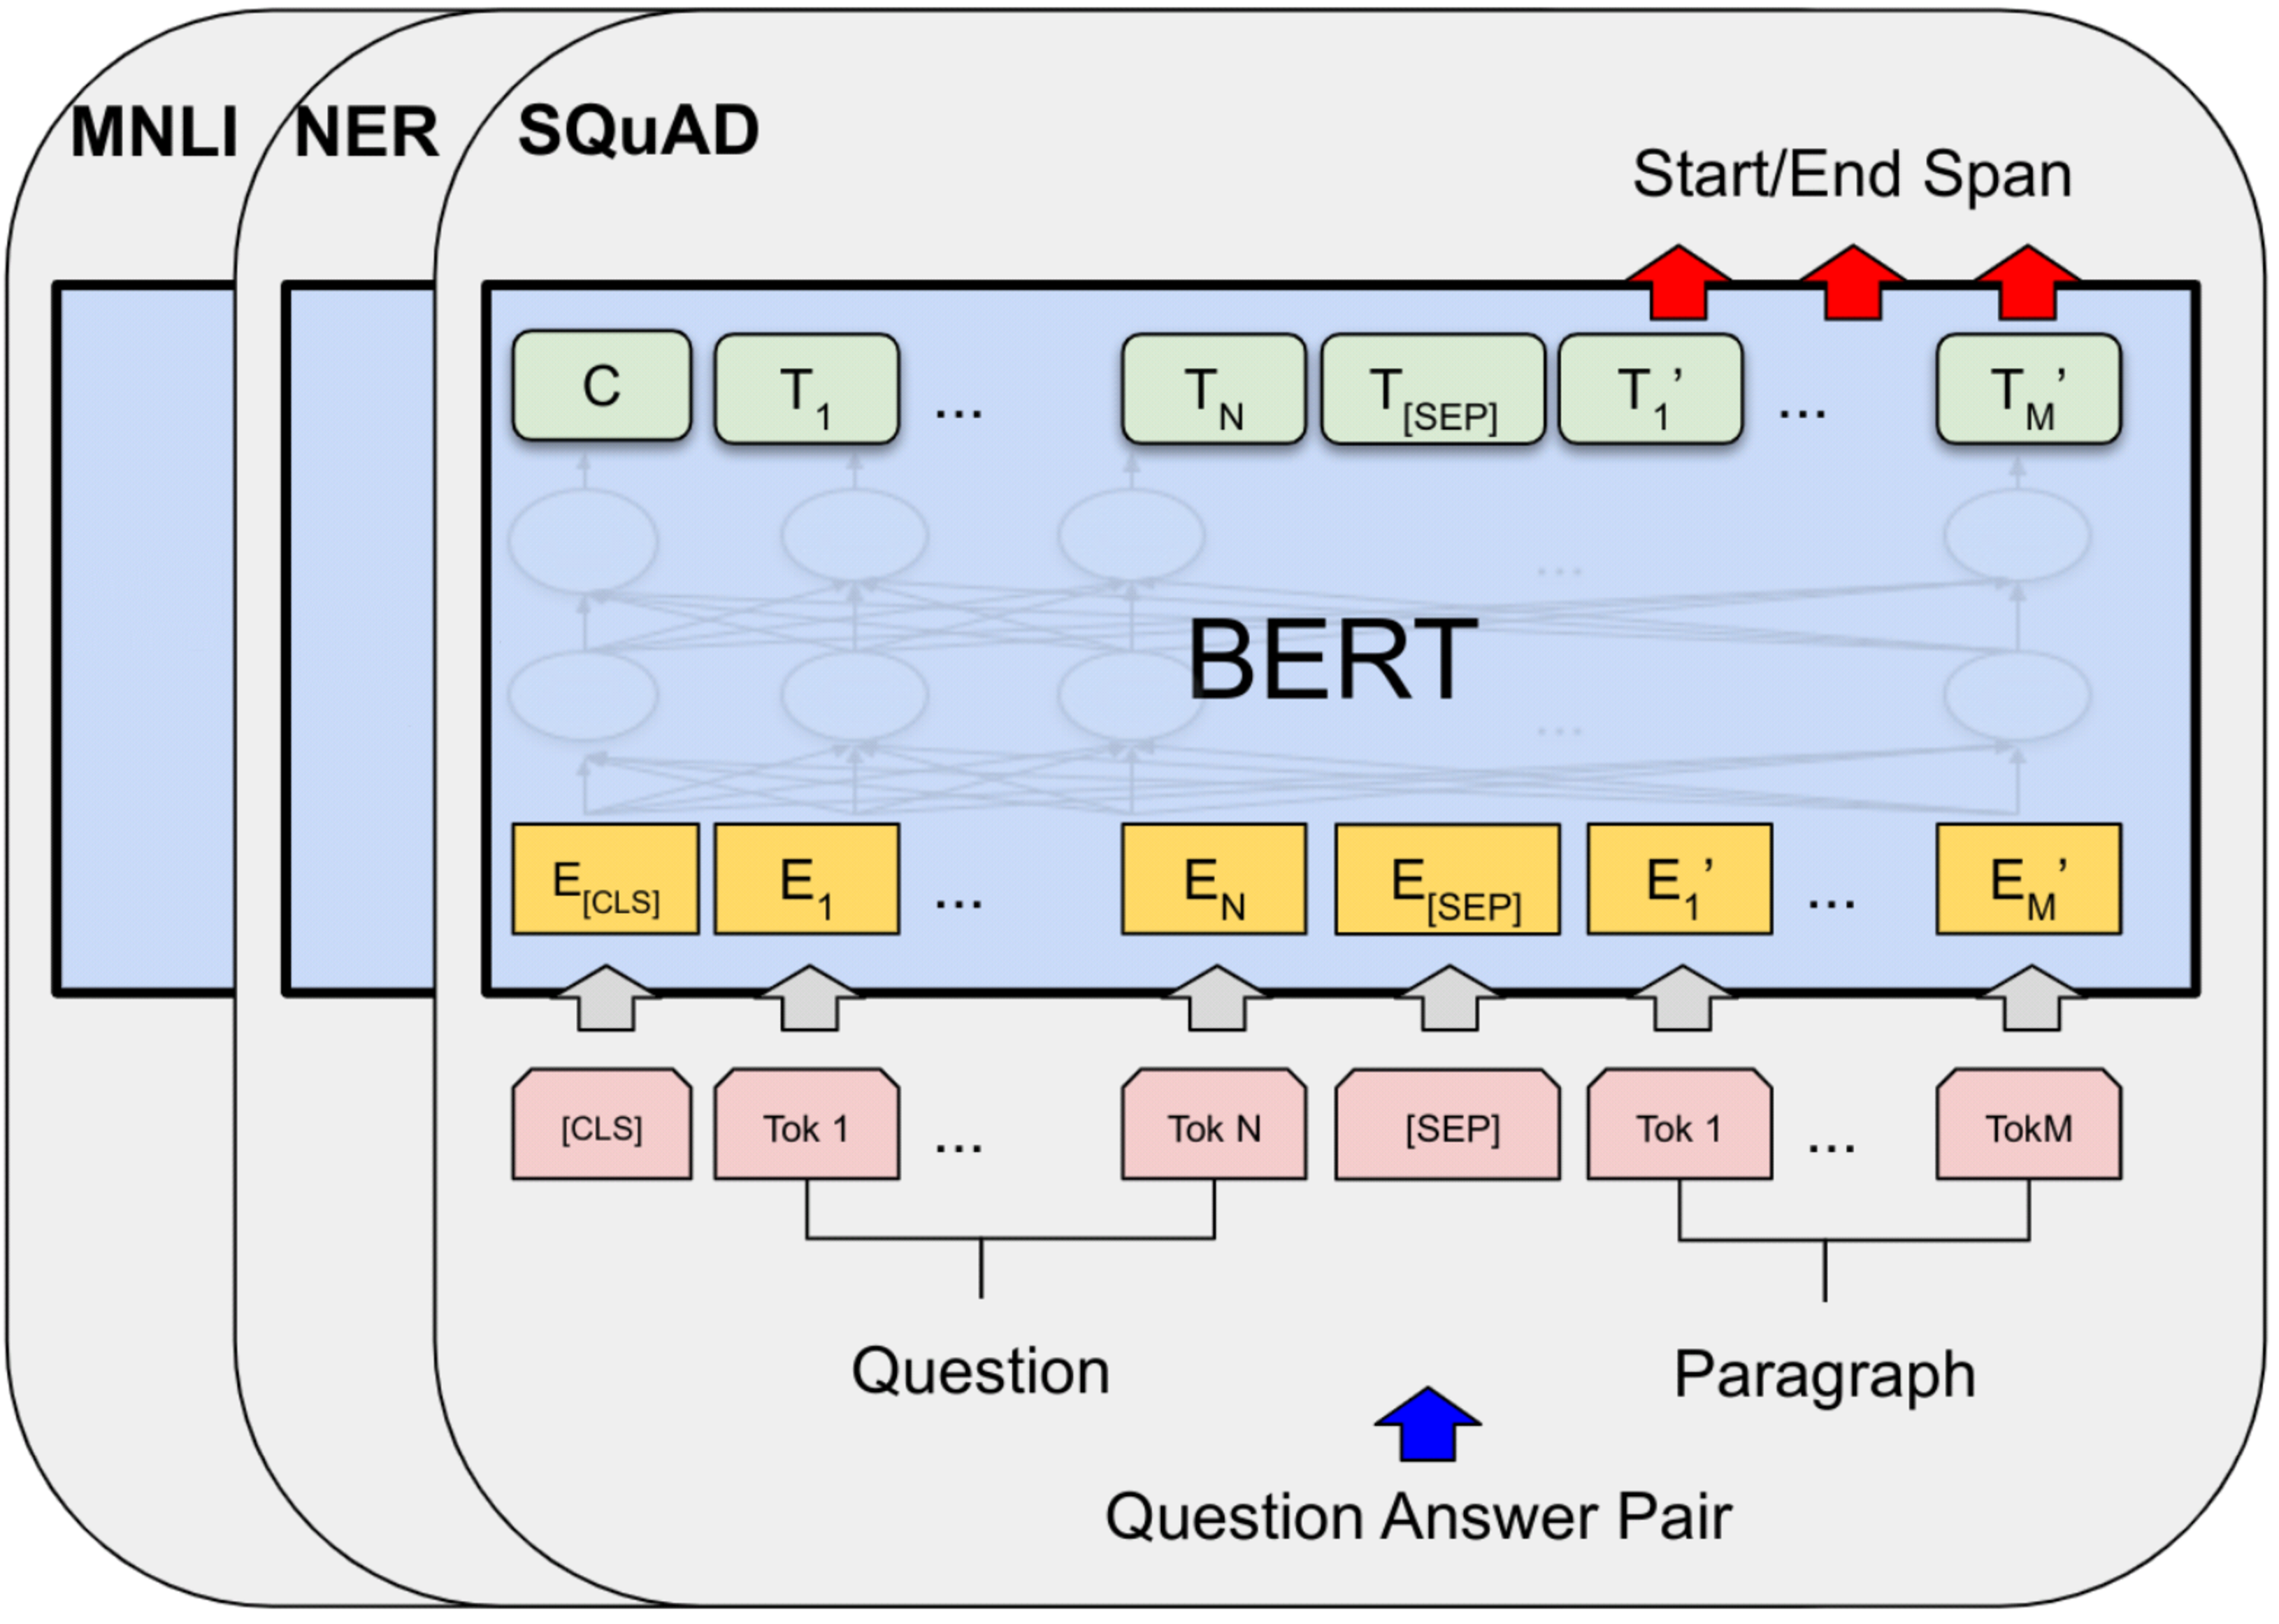
\includegraphics[width=0.7\textwidth]{img/embedders/bert/fine-tuning}
  \caption{Fine-Tuning for SQuAD.}
  \source{\textsc{Devlin} et al. -- BERT}
  \label{fig:bert:fine-tuning}
\end{figure}

In Figure \ref{fig:bert:fine-tuning}, the fine-tuning of the model for SQuAD
takes as input sequence a question and a paragraph containing the answer to this
question. Regarding the model's output for this NLP task, BERT returns the
answer to a submitted question. For this purpose, BERT highlights the starting
and ending word of a given paragraph that includes the answer to that question
only if that answer is in the paragraph. Therefore, it is interesting to look at
the probability that a word is the start/end of the answer span.

\begin{definition}[Word Probability -- Start/End of the Answer Span]
  Let $S \in \mathbb{R}^H$ be the start vector, $E \in \mathbb{R}^H$ be the end
  vector, $T_i \in \mathbb{R}^H$ be the final hidden vector for the
  i\textsuperscript{th} input token, and $j$ be the position of the ending
  word. Mathematically, the following two equations represent the probability that
  the word $i$ is the start/end of the answer span.
  \begin{equation}
    \mathrm{PS_i} = \frac{e^{ST_i}}{\sum_je^{ST_j}} \qquad \mathrm{PE_i} = \frac{e^{ET_i}}{\sum_je^{ET_j}}
    \label{eq:def:bert:word:probabilities}
  \end{equation}

  where the sum of $ST_i$ and $ET_j$ defines the score of a candidate span from
  position $i$ to position $j$. Afterward, the maximum scoring span where $j \geq
  i$ is used as a prediction.
  \label{def:squad:word:probability}
\end{definition}

The starting and ending tokens containing the answer are determined using the
softmax activation function on the dot product between the output embeddings and
the set of weights. From then on, the word with the highest probability is
assigned as the start word, and the process continues to iterate to determine
the end word. As most hyperparameters are similar to those of the pre-training,
the only new hyperparameters added during the fine-tuning concern a
classification layer. From then on, an exhaustive search of values can be done
to choose the best model according to these hyperparameters.

%%% Local Variables:
%%% mode: latex
%%% TeX-master: "../../report"
%%% End:
